
\section{Exercises}

%%%%%%%%%%%%%%%%%%%%%%%%%%%%%%%%%%%%%

\subsection{An example}

%%%%%%%%%%%%%%%%%%%%%%%%%%%%%%%%%%%%%

{\eoce{A migraine is a common type of headache for which patients frequently use acupuncture. To determine whether acupuncture relieves migraine pain researchers conducted a randomized controlled study where 100 adults suffering from migraine pain were randomly assigned to treatment and control groups (50 in each). Patients in the treatment group received twice-weekly treatment for 12 weeks with an acupuncture program that was specifically designed to treat migraines. Patients in the control group received sham acupuncture (needle insertion at nonacupoint locations). Patients were asked at the end of the study whether or not they experienced improvement in migraine headache. The results are summarized in the contingency table below.
\begin{enumerate}[(a)]
\setlength{\itemsep}{0mm}
\item What percent of patients in the control and treatment groups showed improvement?
\item At a first glance, does acupuncture appear to be effective treatment for migraines?
\item Does the data convince you that there is a real improvement for those patients in the treatment group? Or do you think that the results might just be due to chance?
\end{enumerate}
\begin{center}
\begin{tabular}{ll  cc c} 
			&				& \multicolumn{2}{c}{\textit{Improvement}} \\
\cline{3-5}
			&				& No 		& Yes 	& Total	\\
\cline{2-5}
							&Control 		& 22	 	& 28		& 50 	\\
\raisebox{1.5ex}[0pt]{\emph{Group}}	&Treatment	& 15	 	& 35 	 	& 50 \\
\cline{2-5}
							&Total		& 37		& 63		& 100
\end{tabular}
\end{center}
}
{
\begin{enumerate}[(a)]
\item Percent who showed improvement in the treatment group: $35/50 = 0.70 \rightarrow 60\%$. \\
Percent who showed improvement in the control group: $28/50 = 0.56 \rightarrow 56\%$. \\
\item While 70\% of the patients in the treatment group showed improvement, only 56\% of the patients who got the sham treatment (control) showed improvement. There is a 14\% difference between the improvement rates in the two groups. It appears that patients in the treatment group are more likely to show improvement and hence at a first glance, acupuncture appears to be an effective treatment for migraine.
\item Even if acupuncture was not an effective treatment for migraine, typically we would not get the exact same improvement rate in each group. Maybe the difference of 14\% was just due to chance. However, our analysis does not indicate whether what we are seeing is real or a natural fluctuation. 
\end{enumerate}
}}

%

{\eoce{A survey was conducted to study the smoking habits of UK residents \citep{data:smoking}. The table below shows how many of the males and females are smokers.
\begin{center}
\begin{tabular}{ll  cc} 
			&	\multicolumn{1}{c}{}	& \multicolumn{2}{c}{\textit{Gender}} \\ 
\cline{3-4} 
			&		& Female 	& Male 	\\
\cline{2-4}
							&No	 	& 731 	& 539 	\\
\raisebox{1.5ex}[0pt]{\emph{Smoke}}	&Yes	& 234 	& 187 	\\
\cline{2-4}
\end{tabular}
\end{center}
\begin{enumerate}[(a)]
\setlength{\itemsep}{0mm}
\item What percent of males and females smoke?
\item At a first glance, does gender and smoking appear to be related?
\item Does the data convince you that there is a real relationship between gender and smoking? Or do you think that the results might just be due to chance?
\end{enumerate}
}
{
\begin{enumerate}
\item[(a)] Percentage of women who smoke: $\frac{234}{234+731} \approx 0.24 \rightarrow 24\%$ \\
Percentage of men who smoke: $\frac{234}{234+731} \approx 0.26 \rightarrow 26\%$
\item[(b)] 24\% of women and 26\% of men smoke. Even though these percentages are not equal, they are very close. So the 2\% difference might just be a natural fluctuation, which would mean that gender and smoking are independent. In Chapter 4 we will discuss further how close is close enough to say that independence is reasonable.
\item[(c)] The 2\% difference between the male and female smokers might also be an actual difference, which would mean that gender does have an effect on whether or not people choose to smoke. However, our analysis does not indicate whether what we are seeing is real or a natural fluctuation.
\end{enumerate}
}\label{UKSmoking_maleFemaleSmoker}
}

%%%%%%%%%%%%%%%%%%%%%%%%%%%%%%%%%%%%%

\subsection{Data basics}

%%%%%%%%%%%%%%%%%%%%%%%%%%%%%%%%%%%%%

{\textit{In Exercises~\eoceref{airpollutionSoCalPregnancy} to~\eoceref{Prop23} identify \begin{enumerate}[(a)]
\setlength{\itemsep}{0mm}
\item the cases studied,
\item the variables studied and their types, and
\item the main research question of the study.
\end{enumerate}}
}

{\eoce{Researchers collected data to examine the relationship between pollutants and preterm births in Southern California. Measurements of carbon monoxide (CO), nitrogen dioxide, ozone, and particulate matter less than 10$\mu$m (PM$_{10}$) at air-quality-monitoring stations were used to create exposure of estimates for periods of pregnancy. Birth weight data was also collected on 143,196 births between the years 1989 and 1993. The analysis suggested that increased ambient PM$_{10}$ and, to a lesser degree, CO concentrations may contribute to the occurrence of preterm births. \citep{Ritz+Yu+Chapa+Fruin:2000}}
{
\begin{enumerate}[(a)]
\item The cases are 143,196 eligible study subjects who were singletons born between 1989 and 1993.
\item The variables are measurements of carbon monoxide (CO), nitrogen dioxide, ozone, and particulate matter less than 10$\mu$m (PM$_{10}$) collected at air-quality-monitoring stations as well as the birth weights of the babies. All of these variables are continuous numerical variables.
\item The research question was ``Does air pollution exposure have an effect on preterm births?"
\end{enumerate}
}\label{airpollutionSoCalPregnancy}
}

%

{\eoce{The Buteyko method is a shallow breathing technique developed by Konstantin Buteyko, a Russian doctor, in 1952. Anecdotal evidence suggests that the Buteyko method can reduce asthma symptoms and improve quality of life. In a study aimed to determine the effectiveness of this method, 600 adult patients aged 18-69 years diagnosed and currently treated for asthma were divided into two groups. One group practiced the Buteyko method and the other did not. Patients were scored on quality of life, activity, asthma symptoms and medication reduction on a scale from 0 to 10. On average the participants in the Buteyko group experienced a significant improvement in asthma with a reduction in symptom and medication and improvement in quality of life. \citep{McDowan:2003}}
{
\begin{enumerate}[(a)]
\item The cases are 600 adult patients aged 18-69 years diagnosed and currently treated for asthma. 
\item The variables were whether or not the patient practiced the Buteyko method (categorical) and measures of quality of life, activity, asthma symptoms and medication reduction of the patients (numerical, discrete).
\item The research question was ``Do asthmatic patients who practice the Buteyko method experience improvement in their condition?".
\end{enumerate}
}\label{buteykoAsthma600Patients}
}

%

{\eoce{Definition of obesity is based on body fat percentage (more than 35\% body fat for women and more than 25\% for men), however measuring body fat percentage accurately is difficult. Therefore body mass index (BMI),  ratio of height and weight squared,  is often used as an alternative indicator for obesity. A common criticism of BMI is that it assumes the same relative fatness regardless of age, sex, or ethnicity. In order to determine how useful BMI is for predicting body fatness across age, sex and ethnic groups, researchers studied 202 black and 504 white men and women who resided in or near New York City, were ages 20-94 years, and had BMIs of 18-35 kg/m$^2$. Participants reported their age, sex and ethnicity and were measured for weight, height, waist and hip circumference and length of tibia. Body density and volume were determined by submerging the participants in water, and total body water was determined using blood testing. These measurements were used for calculating body fat percentage and fat free body mass.  \citep{Gallagher:1996} 
}
{
\begin{enumerate}[(a)]
\item The cases are 202 black and 504 white men and women who resided in or near New York City, were ages 20-94 years, and had BMIs of 18-35 kg/m$^2$.
\item The variables are age (numerical, continuous), sex (categorical), ethnicity (categorical), weight, height, waist and hip circumference, length of tibia, body density and volume, total body water, body fat percentage, fat free body mass (numerical, continuous). 
\item The research question was ``How useful is BMI for predicting body fatness across age, sex and ethnic groups?".
\end{enumerate}
}\label{BMIAgeSexEth}
}

%

{\eoce{A social scientist interested in the relationship between certain characteristics of voters and support for Proposition 23 conducted a survey before the 2010 midterm election on 1000 registered California voters. If enacted by voters this proposition would freeze the provisions of California's clean air legislation. Along with whether or not they support Prop 23, respondents in this survey were asked their age, race, gender, highest degree earned, occupation, income, party affiliation, how many cars they own and whether or not they own an alternative fuel vehicle (hybrid, biodiesel, etc.). 
}
{
\begin{enumerate}[(a)]
\item The cases are 1000 California votes registered to vote in the 2010 midterm election.
\item The variables are whether or not they support Proposition 23 (categorical), age (numerical, continuous), race, gender, highest degree earned, occupation (categorical), income (numerical, continuous), party affiliation (categorical), how many cars they own (numerical, discrete) and whether or not they own an alternative fuel vehicle (categorical).
\item The research question was ``What are certain characteristics of California voters who do and do not support Proposition 23?"
\end{enumerate}
}\label{Prop23}
}

%

\eoce{Exercise~\eoceref{UKSmoking_maleFemaleSmoker} introduced a study about the smoking habits of UK residents. Below is a data matrix displaying a portion of the data collected in this survey.
\begin{table}[h]
\begin{center}
\scriptsize{
\begin{tabular}{rccccccc}
  \hline
 & gender & age & maritalStatus & grossIncome & smoke & amtWeekends & amtWeekdays \\ 
  \hline
1 & Female &  42 & Single & Under $\pounds$2,600 & Yes &  12 cig/day &  12 cig/day \\ 
2 & Male &  44 & Single & $\pounds$10,400 to $\pounds$15,600 & No & N/A & N/A \\ 
3 & Male &  53 & Married & Above $\pounds$36,400 & Yes &   6 cig/day &   6 cig/day \\ 
\vdots & \vdots &  \vdots & \vdots & \vdots & \vdots & \vdots & \vdots \\ 
1691 & Male &  40 & Single & $\pounds$2,600 to $\pounds$5,200 & Yes &   8 cig/day &   8 cig/day \\   
   \hline
\end{tabular}
}
\end{center}
\end{table}
\begin{enumerate}
\setlength{\itemsep}{0mm}
\item[(a)] What does each row of the data matrix represent?
\item[(b)] How many participants were included in the survey?
\item[(c)] Identify the variables in the data set and give a short description of what each variable represents. 
\end{enumerate}
}
{
\begin{enumerate}
\item[(a)] Each row of the data matrix represents an observation, i.e. a participant in the survey.
\item[(b)] There are 1,691 participants in the survey.
\item[(c)] The table below lists the variables in the data set and gives a short description of each variable:
\begin{center}
\begin{tabular}{l l}
  \hline
\textbf{variable} & \textbf{description} \\ 
\hline
gender & gender of the participant \\ 	
age & age of the participant (in years) \\
maritalStatus & marital status of the participant \\
grossIncome & gross income of the participant (in $\pounds$) \\
smoke & whether or not the participant smokes \\
amtWeekends & number of cigarettes smoked on weekend (\# of cigarettes / day) \\ 
amtWeekdays & number of cigarettes smoked on a week day (\# of cigarettes / day) \\
  \hline
\end{tabular}
\end{center}
\end{enumerate}
}\label{UKSmoking_datamatrix}

%

\eoce{Sir Ronal Aylmer Fisher was an English statistician, evolutionary biologist and geneticist who worked on a data set that contained sepal length and width and petal length and width from three species of iris flowers (setosa, versicolor and virginica). There were 50 flowers from each species in the data set \citep{Fisher:1936}.
\begin{center}
\begin{minipage}[c]{0.55\textwidth}
\begin{enumerate}
\setlength{\itemsep}{0mm}
\item[(a)] How many cases were included data?
\item[(b)] How many numerical variables are included in the data? Indicate what they are and if they are continuous or discrete.
\item[(c)] How many numerical variables are included in the data and what are they? How many levels does each have, and what are they? Are they also ordinal?
\item[]\vspace{-2mm}
\item[]\tiny{Iris versicolor. Photocredits: rtclauss on Flickr.} \\
\tiny{http://www.flickr.com/photos/rtclauss/3834965043/}
\end{enumerate}
%\vspace{3mm}
\end{minipage}
\begin{minipage}[c]{0.4\textwidth}
\begin{center}
\includegraphics[width = 30mm]{01/figures/eoce/irisVersicolor}
\end{center}
\end{minipage}
\end{center}
}
{
\begin{enumerate}
\item[(a)] There are 50 * 3 = 150 cases included in this data set.
\item[(b)] There are 4 numerical variables in the data: sepal length, sepal width, petal length and petal width and they are all continuous numerical variables.
\item[(c)] There is only one categorical variable in the data, which is species. It has 3 levels: setosa, versicolor, virginica. It is not an ordinal variable.
\end{enumerate}
}

%

\eoce{Exercise~\eoceref{UKSmoking_maleFemaleSmoker} introduced a study about the smoking habits of UK residents. Indicate if the variables in the study are numerical or categorical. If numerical, identify as continuous or discrete.}
{
\begin{center}
\begin{tabular}{l l}
  \hline
\textbf{variable} & \textbf{type} \\ 
\hline
gender & categorical \\ 	
age & numerical, continuous \\
maritalStatus & categorical \\
grossIncome & categorical \\
smoke & categorical \\
amtWeekends & numerical, discrete \\ 
amtWeekdays & numerical, discrete \\
  \hline
\end{tabular}
\end{center}
}

%%%%%%%%%%%%%%%%%%%%%%%%%%%%%%%%%%%%%

\subsection{Examining numerical data}

%%%%%%%%%%%%%%%%%%%%%%%%%%%%%%%%%%%%%

\eoce{Data has been collected on life spans (in years) and gestation lengths (in days) for 62 mammals \citep{Allison+Cicchetti:1975}. A scatter plot of life span vs. length of gestation is shown below.
\begin{enumerate}
\setlength{\itemsep}{0mm}
\item[(a)] What type of an association is apparent between life span and length of gestation?
\item[(b)] What type of an association would you expect to see if the axes of the plot were reversed, i.e. if we plotted length of gestation vs. life span?
\item[(c)] Are life span and length of gestation independent? Explain your reasoning.
\end{enumerate}
\begin{center}
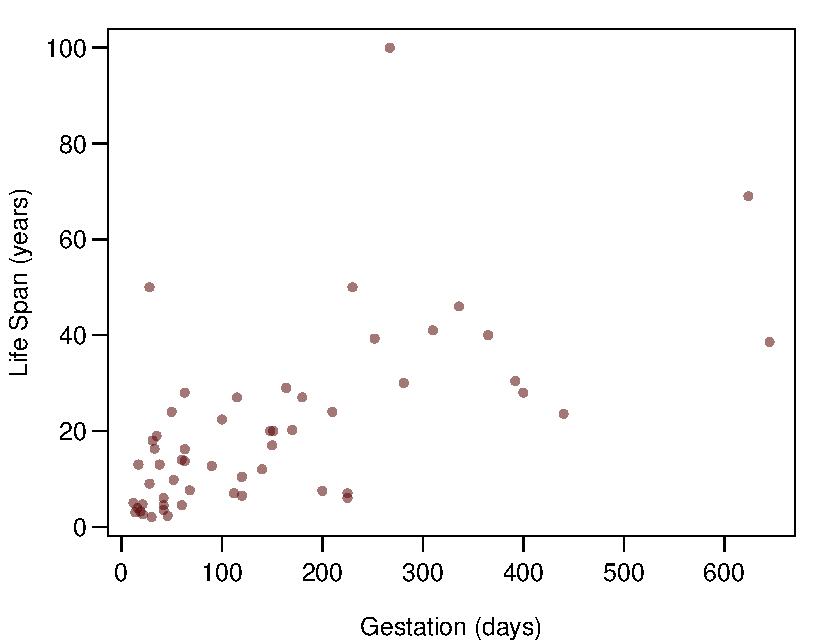
\includegraphics[width = 60mm]{01/figures/eoce/LifeSpanvsGest.pdf}
\end{center}
}
{\begin{enumerate}
\item[(a)] There is a positive and linear association between life span and gestation, meaning that mammals with longer gestation periods tend to live longer as well.
\item[(b)] The association would still be positive; if as length of gestation increases life span is expected to increase, then as life span increases, length of gestation is expected to increase as well.
\item[(c)] No, they are not independent since there is a clear association between the two variables.
\end{enumerate}
}

%

\eoce{Office productivity is relatively low when the employees feel no stress about their work or job security. However high levels of stress can also lead to reduced employee productivity. Sketch a plot to represent the relationship between stress and productivity and explain your reasoning.}
{
\begin{center}
\begin{minipage}[c]{0.55\textwidth}
A horse shoe shaped association - we would expect productivity to increase as stress increases, but up to a point, after that productivity would decrease as stress continued to increase.
\end{minipage}
\begin{minipage}[c]{0.4\textwidth}
\begin{center}
\includegraphics[width = 40mm]{01/figures/eoce/StressProductivity.pdf}
\end{center}
\end{minipage}
\end{center}
}

%
\pagebreak

\eoce{Indicate which of the below plots show a 
\begin{center}
\begin{minipage}[b]{0.4\textwidth}
\begin{enumerate}
\setlength{\itemsep}{1mm}
\item[(a)] linear association
\item[(b)] non-linear association
\item[(c)] positive association
\item[(d)] negative association
\item[(e)] no association
\end{enumerate}
Each part may refer to more than one plot.
\vspace{10mm}
\end{minipage}
\begin{minipage}[b]{0.5\textwidth}
%\begin{center}
\includegraphics[width = \textwidth]{01/figures/eoce/AssociationPlots.pdf}
%\end{center}
\end{minipage}
\end{center}
}
{
\begin{enumerate}
\item[(a)] (1) and (4)
\item[(b)] (3)
\item[(c)] (1) and (3)
\item[(d)] (4)
\item[(e)] (2)
\end{enumerate}
}

%

\eoce{Identify which value represents the sample mean and which value represents the claimed population mean.
\begin{enumerate}
\setlength{\itemsep}{0mm}
\item[(a)] A recent article in a college newspaper stated that college students get an average of 5.5 hrs of sleep each night. A student who was skeptical about this value decided to conduct a survey on a random sample of 25 students which yielded an average of 6.25 hrs of sleep.
\item[(b)] American households spent an average of about \$52 in 2007 on Halloween merchandise such as costumes, decorations and candy. To see if this number has changed, researchers conducted a new survey in 2008 on 1,500 households and found that in the average amount a household spent on Halloween was \$58.
%\item[(c)] An SAT prep agency claims that their students do significantly better on the SAT as the average score of their students was 1,680 while generally SAT scores have a mean of about 1,520.
\end{enumerate}
}
{
\begin{enumerate}
\item[(a)] Population mean, $\mu_x = 5.5$; sample mean, $\bar{x} = 6.25$.
\item[(b)] Population mean, $\mu_x = 52$; sample mean, $\bar{x} = 58$.
%\item[(c)] Population mean, $\mu_x = 1,520$; sample mean, $\bar{x} = 1,680$.
\end{enumerate}
}

%

\eoce{A random sample from the data set introduced in Exercise~\eoceref{UKSmoking_maleFemaleSmoker} is given. Find the mean for each of the variables listed and mark it on the dot plot of the variable. If you cannot calculate the mean for a variable, indicate why.
\begin{table}[h]
\begin{center}
\footnotesize{
\begin{tabular}{ccccccc}
  \hline
gender & age & maritalStatus & grossIncome & smoke & amtWeekends & amtWeekdays \\ 
  \hline
Female &  51 & Married & 2,600 to 5,200 & Yes &  20 &  20 \\ 
  Male &  24 & Single & 10,400 to 15,600 & Yes &  20 &  15 \\ 
  Female &  33 & Married & 10,400 to 15,600 & Yes &  20 &  10 \\ 
  Female &  17 & Single & 5,200 to 10,400 & Yes &  20 &  15 \\ 
  Female &  76 & Widowed & 5,200 to 10,400 & Yes &  20 &  20 \\ 
   \hline
\end{tabular}
}
\end{center}
\end{table}
}
{
Means for the numerical variables are calculated below. Means are not calculated for gender, marital status, gross income and smoke since those are categorical variables.
\begin{align*}
\bar{x}_{age} &= \frac{51 + 24 + 33 + 17 + 76}{5} = 40.2 \\
\bar{x}_{amtWeekends} &= \frac{20 + 20 + 20 + 20 + 20}{5} = 20 \\
\bar{x}_{amtWeekdays} &= \frac{20 + 15 + 10 + 15 + 20}{5} = 16
\end{align*}
\begin{center}
\includegraphics[width=49mm]{01/figures/eoce/SmokingSample5AgeDotPlot.pdf}
\includegraphics[width=49mm]{01/figures/eoce/SmokingSample5AmtWkendDotPlot.pdf}
\includegraphics[width=49mm]{01/figures/eoce/SmokingSample5AmtWkdayDotPlot.pdf}
\end{center}
}\label{UKSmokingSample5}

%

\eoce{In a class of 25 students, 24 of them take an exam in class and 1 student takes a make-up exam the next day. The professor grades the first batch of 24 exams and finds that the average score is 74 with a standard deviation of 8.9. The student who takes the make-up the next day scores an 64 on the exam.
\begin{enumerate}[(a)]
\setlength{\itemsep}{0mm}
\item Will the average score increase or decrease? What will the revised average score be?
\item Will the standard deviation of the data increase or decrease?
\end{enumerate}
}
{
\begin{enumerate}[(a)]
\item We are given that
\[ n = 24,\quad \bar{x} = 74,\quad s_x = 8.9 \]
Since the new score is smaller than the mean of the 24 previous scores, the new mean should be smaller than the old mean.
\begin{align*}
\bar{x} &= \frac{x_1 + x_2 + \dots + x_{24}}{24} = 74\\
x_1 + x_2 + \dots + x_{24} &= 74 * 24 = 1776\\
x_1 + x_2 + \dots + x_{24} + x_{25} &= 1776 + 64 = 1840\\
\bar{x}_{new} &= \frac{x_1 + x_2 + \dots+x_{24} + x_{25}}{25}=\frac{1840}{25}
= 73.6
\end{align*}
\item The new score, $x_{25}$, is more than 1 standard deviation away from the previous mean, and this will tend to increase the standard deviation of the data. While possible, it is mathematically rather tedious to calculate the new standard deviation.
\end{enumerate}
}

%

\eoce{At a particular mining plant workers on average get 35 paid days off, which is lower than the countrywide average. The manager of this plant is under pressure from a union to increase the number of days workers get paid time off but he does not want to give more days off to the workers since that would be costly. Instead he decides to fire 10 employees and thereby raise the average number of days off. In order to achieve this goal, should he fire employees who have the most number of days off, least number of days off, or those who have about the average number of days off?
}
{
In order to increase the average number of days off, the manager should fire any 10 employees whose average number of days off is between the minimum and the mean number of days off for the entire workforce at this plant. However, firing the 10 employees with the minimum number of days off will have the biggest impact on the average.
}

%

\eoce{Exercise~\eoceref{UKSmoking_maleFemaleSmoker} introduces a data set on the smoking habits of UK residents. Below are histograms displaying the distributions of amount of cigarettes smoked on weekdays and on weekends. Describe the two distributions and compare them.
\begin{center}
\includegraphics[width = 80mm]{01/figures/eoce/AmtWeekendWeekdayHist.pdf}
\end{center}
}
{The distribution of amount of cigarettes smoked on weekends and on weekdays are both right skewed. The values range from 0 to 60 for weekends and from 0 to 55 for weekdays. We can also see that there are more respondents who smoke only a few cigarettes (0 to 5) on the weekdays, about 80 people, than on weekends, about 60 people. Another feature that is visible from the histograms are peaks at 10 and 20 cigarettes. This may be because most people do not keep track of exactly how many cigarettes they smoke, but round their answers to half a pack (10 cigarettes) or a whole pack (20 cigarettes). Due to these peaks the distributions could be classified as bimodal.}

%

\eoce{Below are the final scores of 20 introductory statistics students.
\begin{center}
79, 83, 57, 82, 94, 83, 72, 74, 73, 71, \\
66, 89, 78, 81, 78, 81, 88, 69, 77, 79
\end{center}
Draw a histogram of these data and describe the distribution.
}
{
In order to draw a histogram we first need create a frequency distribution table.
\begin{center}
\begin{minipage}[c]{0.4\textwidth}
\begin{tabular}{cr}
Score & Frequency \\
\hline
55 - 59	& 1 \\
60 - 64	& 0 \\
65 - 69	& 2 \\
70 - 74	& 4 \\
75 - 79	& 5 \\
80 - 84	& 5 \\
85 - 89	& 2 \\
90 - 95	& 1 \\
\hline
Total & 20
\end{tabular}
  \end{minipage}
\begin{minipage}[c]{0.4\textwidth}
\includegraphics[height = 50mm]{01/figures/eoce/StatsFinalScoresHist.pdf} 
\end{minipage}
\end{center}
The distribution is unimodal and symmetric with a mean at 77.7. The values range from 57 to 94. About 80\% of scores are within 10 scores of the mean (between 68 and 88).
}\label{introStatsFinalScores}

%

\eoce{Find the standard deviation of the amount of cigarettes smoked on weekdays and on weekends by the 5 randomly sampled UK residents given in Exercise~\eoceref{UKSmokingSample5}. Is the variability higher on weekends or on weekdays?}
{\begin{align*}
s^2_{amtWeekends} &= \frac{(20 - 20)^2 + (20 - 20)^2 + (20 - 20)^2 + (20 - 20)^2 + (20 - 20)^2}{5 - 1}  = 0 \\
s_{amtWeekends} &= \sqrt{0} = 0 \\
s^2_{amtWeekdays} &= \frac{(20 - 16)^2 + (15 - 16)^2 + (10 - 16)^2 + (15 - 16)^2 + (20 - 16)^2}{5 - 1} = 17.5 \\
s_{amtWeekdays} &= \sqrt{562.7} = 4.18 \\
\end{align*}
Standard deviation for the weekends is 0 while it is 4.18 for the weekdays. Therefore, in our sample, the variability of the amount of cigarettes smoked is higher on weekdays than on the weekends.
}

%

\eoce{A factory quality control manager decides to investigate the percentage of defective items produced each day. Within a given work week (Monday through Friday) the percentage of defective items produced was 2\%, 1.4\%, 4\%, 3\%, 2.2\%.
\begin{enumerate}[(a)]
\setlength{\itemsep}{0mm}
\item Calculate the mean for these data.
\item Calculate the standard deviation for these data, showing each step in detail.
\end{enumerate}
}
{
\begin{enumerate}[(a)]
\item Mean: $ \bar{x} = \frac{2 + 1.4 + 4 + 3 + 2.2}{5} = \frac{12.6}{5} = 2.52 $
\item Variance: $ s_x^2 =\frac{(2 - 2.52)^2+ (1.4 - 2.52)^2 + (4 - 2.52)^2 + (3 - 2.52)^2 + (2.2 - 2.52)^2}{5 - 1} = \frac{4.048}{4} = 1.012 $ \\
Standard deviation: $s_x = \sqrt{1.012} = 1.006 $
\end{enumerate}
}

%

\eoce{Find the median in following data sets.
\begin{enumerate}
\setlength{\itemsep}{0mm}
\item[(a)] 3, 5, 6, 7, 9
\item[(b)] 3, 5, 6, 7, 9, 10
\end{enumerate}
}
{
\begin{enumerate}
\item[(a)] Median: 6
\item[(b)] Median: $\frac{6+7}{2} = 6.5$
\end{enumerate}
}

%

{\eoce{Find the median in following data sets.
\begin{enumerate}
\item[(a)] -1,  6,  8, -2, -9, -3,  4, -3,  3
\item[(b)] 6, 6, -5, -5,  7,  1,  4,  0,  8, -8
\end{enumerate}
}
{
\begin{enumerate}
\item[(a)] First we must put the data in ascending order: $-9, -3,  -3,  -2, -1,  3,  4, 6,  8$. Median: -1
\item[(b)] First we must put the data in ascending order: $-8, -5, -5,  0,  1,  4,  6,  6,  7,  8$. Median: $\frac{1+4}{2} = 2.5$
\end{enumerate}
}}

%

\eoce{Below is the five number summary for the  final exam scores data given in Exercise~\eoceref{introStatsFinalScores}. Create a box plot of the data based on these values.
\begin{center}
\begin{tabular}{r|l}
Min & 57 \\
Q1 & 72.5 \\
Q2 (Median) & 78.5 \\
Q3 & 82.5 \\
Max & 94 \\
\end{tabular}
\end{center}
}
{
\begin{itemize}
\item The box goes from Q1 (72.5) to Q3 (82.5), the line inside the box is the median (78.5).
\item Below is how we determine where the whiskers go and check for outliers:
\begin{align*}
\text{IQR} &= Q3 - Q1 = 82.5 - 72.5 = 10 \\
\text{Upper Fence} &= Q3 + 1.5 * IQR = 82.5 + 1.5 * 10 = 97.5 \\
\text{Lower Fence} &= Q1 - 1.5 * IQR = 72.5 - 1.5 * 10 = 57.5
\end{align*}
\end{itemize}

\begin{center}
\begin{minipage}[c]{0.47\textwidth}
\begin{itemize}
\item Any point above the UF is an outlier: none \\
Any point below the LF is an outlier: 57
\item Since there is an outlier on the lower end, the lower whisker goes till the last point above the LF: 66 \\
Since there is no outlier on the upper end, the upper whisker goes till the maximum: 94
\end{itemize}
\end{minipage}
\begin{minipage}[c]{0.45\textwidth}
\hspace{10mm} \includegraphics[width = 60mm]{01/figures/eoce/StatsFinalScoresBoxplot.pdf}
\end{minipage}
\end{center}
}

%

\eoce{According to a study on Twitter usage published by the Harvard Business Review, the median number of tweets per day is 0.01. 25\% of users have 0 tweets per day while the top 25\% of users have 0.37 tweets per day \citep{web:hbrTwitter}. Justin Bieber's on average tweets 14.3 times per day \citep{web:yahooNewsBiebs}. Is he considered an outlier? Explain.}
{
First we calculate the upper fence:
\begin{align*}
IQR &= Q3 - Q1 = 0.37 - 0 = 0.37 \\
UF &= Q3 + 1.5 * IQR = 0.37 + 1.5 * 0.37 = 0.925 \\
\end{align*}
Since Justin Bieber's average number of tweets per day is above the upper fence, he is in fact considered an outlier.
}

%

\noindent\begin{minipage}[c]{0.35\textwidth}
\eoce{Describe the distribution in the following histograms and match them to the box plots. \vspace{62mm}}
{
\begin{enumerate}
\item[(a)] The distribution is unimodal and symmetric with a mean around 60. The values range from 50 to 75. This matches the box plot (2) which also shows a symmetric distribution in this range.
\item[(b)] The distribution is uniform and values range from 0 to 100. This matches box plot (3) which shows a symmetric distribution in this range. Also, each 25\% chunk of the box plot have about the same width and there are no suspected outliers.
\item[(c)] The distribution is unimodal and right skewed with a median between 1 and 2. The values range from 0 to 7. This matches box plot (1) which also shows a right skewed distribution in this range.
\end{enumerate}
}
\end{minipage}
\begin{minipage}[c]{0.64\textwidth}
\begin{center}
\includegraphics[width = 0.99\textwidth]{01/figures/eoce/HistBoxMatch}
\end{center}
\end{minipage}
%

\noindent\begin{minipage}[c]{0.34\textwidth}
\eoce{Compare the two plots given below. What characteristics of the distribution are apparent in the histogram and not in the box plot? What characteristics are apparent in the box plot but not in the histogram? \vspace{41mm}
}
{
The histogram shows that the distribution is bimodal while this is not apparent in the box plot. On the other hand the box plot makes it easy to identify the outliers whereas looking at the histogram it is difficult to tell if the higher values are outliers or not.
}
\end{minipage}
\begin{minipage}[c]{0.65\textwidth}
\begin{center}
\includegraphics[width = 0.9\textwidth]{01/figures/eoce/BiModHistBoxPlot.pdf}
\end{center}
\end{minipage}

%

{\eoce{Infant mortality rate is defined as the number of deaths of infants under one year old in a given year per 1,000 live births in the same year. This rate is often used as an indicator of the level of health in a country. The histogram below shows the distribution of 2010 infant death rates of 224 countries as provided by the CIA fact book \citep{data:ciaFactBookInfMort:2010}. 
\noindent\begin{minipage}[c]{0.35\textwidth}
\begin{enumerate}[(a)]
\item Based on this histogram, estimate the median, Q1 and Q3.
\item Would you expect the mean of this data set to be smaller or larger than the median? Explain your reasoning.
\end{enumerate}
\end{minipage}
\begin{minipage}[c]{0.64\textwidth}
\begin{center}
\includegraphics[width = 0.9\textwidth]{01/figures/eoce/infMortRate.pdf}
\end{center}
\end{minipage}
}
{
\begin{enumerate}[(a)]
\item Since median is defined as the $50^{th}$ percentile and about 50\% of the data is in the first bar, we would expect median to be between 0 and 20. Q1 is also between 0 and 20 as the $25^{th}$ percentile is in the first bar as well. Q3, defined as the $75^{th}$ percentile, is located between 40 and 60.
\item We would expect the mean to be higher than the median. Since the distribution is right skewed will pull the arithmetic average (mean) up.
\end{enumerate}
}
}

%

\eoce{Below are a histogram and box plot of marathon times of male and female New York Marathon runners between 1980 and 1999.  \\
\noindent\begin{minipage}[c]{0.45\textwidth}
\begin{enumerate}[(a)]
\setlength{\itemsep}{5mm}
\item What features of the distribution are apparent in the histogram and not the box plot? What features are apparent in the box plot but not in the histogram?
\item What may be the reason for the bimodal distribution? Explain.
\item Compare the distribution of marathon times for men and women based on the box plots given in the bottom plot.
\item[]
\item[]
\item[]
\item[]
\item[]
\end{enumerate}
\end{minipage}
\begin{minipage}[c]{0.55\textwidth}
\begin{center}
\includegraphics[width=0.9\textwidth]{01/figures/eoce/MarathonHistBox.pdf} \\
\includegraphics[width=0.9\textwidth]{01/figures/eoce/MarathonGender.pdf}
\end{center}
\end{minipage}
}
{
\begin{enumerate}[(a)]

\item From the histogram we can see the the distribution is bimodal. In the box plot the outliers are easier to identify.

\item Gender may be the reason, it is likely that men and women have different average marathon times.

\item The median marathon time for men is about 2.2 hrs while it is about 2.5 hrs for women; therefore, men are faster on average. The minimum marathon time for men is about 2.1 hrs whereas it is about 2.4 hrs for women. The maximum marathon time for men is about 2.5 hrs for men whereas it is about 3.1 hrs for women. Both distributions have outliers on the higher end but what is considered an outlier for men is lower than the third quartile for women.

\end{enumerate}
}\label{NYMarathon}

%

\noindent\begin{minipage}[c]{0.45\textwidth}
\eoce{Take another look at the data presented in Exercise~\eoceref{NYMarathon} using the time series plot below. Describe the trends apparent in the plot and comment on whether or not these trends were apparent in the histogram and/or the box plot.
%\begin{center}
%\includegraphics[width=60mm]{01/figures/eoce/MarathonTimeGender.pdf}
%\end{center}
\vspace{36mm}}
{
It appears that marathon times decreased greatly between 1970-1975 and remained somewhat steady after that time for males and females. Males consistently had shorter marathon times than females throughout the years. The data set contains one marathon time for males and one for females each year. These are most probably the winners of each year's marathon. From the box plots of males and females we could tell that males ran faster ``on average" however we could not tell that the winning male time for each year was better than the winning female time. We also could not tell from the histogram or the box plot that marathon times have been decreasing for males and females throughout the years.
}
\end{minipage}
\begin{minipage}[c]{0.55\textwidth}
\begin{center}
\includegraphics[width=0.95\textwidth]{01/figures/eoce/MarathonTimeGender.pdf}
\end{center}
\end{minipage}
\vspace{2mm}

%

\eoce{Describe whether you expect the distribution to be symmetric, right skewed or left skewed. In each case, specify whether you would use the mean or median to describe the center, and whether you would prefer to use the standard deviation or IQR to describe the spread.
\begin{enumerate}
\setlength{\itemsep}{0mm}
\item[(a)] Housing prices in a country where 25\% of the houses cost below \$350,000, 50\% of the houses  cost below \$450,000, 75\% of the houses cost below \$1,000,000 and there are houses selling at over \$6,000,000.
\item[(b)] Housing prices in a country where 25\% of the houses cost below \$300,000, 50\% of the houses  cost below \$600,000, 75\% of the houses cost below \$900,000 and there no houses selling at over \$1,200,000.
\item[(c)] Number of alcoholic drinks consumed by college students in a given week.
\item[(d)] Annual salaries of the employees of a Fortune 500 company.
\end{enumerate}
}
{
\begin{enumerate}
\item[(a)] The distribution is right skewed with potential outliers on the positive end, therefore median and IQR are appropriate measures of center and spread.
\item[(b)] The distribution is somewhat symmetric and probably does not have outliers, therefore mean and standard deviation appropriate measures of center and spread.
\item[(c)] The distribution is right skewed. There will be some students who do not consume any alcohol but this is the minimum (there cannot be students who consume fewer than 0 drinks). Most students would consume about the median number of drinks, maybe 2-3 drinks, but there will also be a few students who consume a lot more alcohol than that, giving the distribution a long right tail. Due to the skew, median and IQR are appropriate measures of center and spread.
\item[(d)] The distribution is right skewed. Most employees will make about the median salary but we would expect to have some high level executives making a lot more, therefore giving the distribution a long right tail. Due to the skew, median and IQR are appropriate measures of center and spread.
\end{enumerate}
}

%

\eoce{The first histogram below shows the distribution of the yearly incomes of 40 patrons at a coffee shop. Then walks in two friends, one makes \$225,000 per year and the other makes \$250,000. The second histogram shows the new distribution of income. Also provided are summary statistics for the two distributions. \\
\begin{minipage}[c]{0.59\textwidth}
\includegraphics[width=\textwidth]{01/figures/eoce/Salary.pdf}
\end{minipage}
\begin{minipage}[c]{0.4\textwidth}
\begin{center}
\begin{tabular}{r c c}
  \hline
 & (1) & (2) \\ 
  \hline
n & 40 & 42 \\ 
  Min. & 60,420 & 60,420 \\ 
  1st Qu. & 64,450 & 64,610 \\ 
  Median & 65,210 & 65,370 \\ 
  Mean & 65,060 & 73,270 \\ 
  3rd Qu. & 66,290 & 66,320 \\ 
  Max. & 68,320 & 250,000 \\ 
    SD & 1,832 & 37,313 \\ 
   \hline
\end{tabular}
\end{center}
\end{minipage}
\begin{enumerate}
\setlength{\itemsep}{0mm}
\item[(a)] Is the mean or the median a better measure of the typical amount earned by the 42 patrons at this coffee shop? What does this say about the robustness of the two measures.
\item[(b)] Is the standard deviation or the IQR a better measure of variability in the amounts earned by the 42 patrons at this coffee shop? What does this say about the robustness of the two measures.
\end{enumerate}
}
{
\begin{enumerate}
\item[(a)] The median is a much better measure of the typical amount earned by these 42 people. The mean is much higher than what the majority of people make. This is because the mean is simply an arithmetic average and gets effected by the two extreme observations. The median does not get effected as much since it is robust to outliers.
\item[(b)] The IQR  is a much better measure of variability in the amounts earned by these 42 people. The standard deviation gets affected greatly by the two high salaries but the IQR is robust to these extreme observations.
\end{enumerate}
}

%%%%%%%%%%%%%%%%%%%%%%%%%%%%%%%%%%%%%

\subsection{Considering categorical data}

%%%%%%%%%%%%%%%%%%%%%%%%%%%%%%%%%%%%%

\eoce{Below is a relative frequency bar plot and a pie chart showing the distribution of marital status in the data set on the smoking habits of UK residents introduced in Exercise~\eoceref{UKSmoking_maleFemaleSmoker}.
\begin{enumerate}
\setlength{\itemsep}{0mm}
\item[(a)] What features are apparent in the bar plot but not in the pie chart?
\item[(b)] What features are apparent in the pie chart but not in the bar plot?
\item[(c)] Which graph would you prefer to use for displaying categorical data? Consider which graph gives you the most information.
\end{enumerate}
\begin{center}
\includegraphics[width = 0.495\textwidth]{01/figures/eoce/SmokingMarStatBarPlot.pdf}
\includegraphics[width = 0.495\textwidth]{01/figures/eoce/SmokingMarStatPieChart.pdf}
\end{center}
}
{
\begin{enumerate}
\item[(a)] As well as the order of the categories we can also see the relative frequencies in the bar plot. These proportions are not readily available in the pie chart.
\item[(b)] There are no features that are apparent in the pie chart but not in the bar plot.
\item[(c)] We would prefer to use a bar plot as we can also see the relative frequencies of the categories in this graph.
\end{enumerate}
}

%

\eoce{The table below shows the relationship between hair color and eye color for a group of 1,770 German men.
\begin{center}
\begin{tabular}{ll  ccc  r} 
			&	\multicolumn{1}{c}{}	& \multicolumn{3}{c}{\textit{Hair Color}} & \\ 
\cline{3-5}
			&		& Brown 	& Black 	& Red	& Total  \\
\cline{2-6}
\textit{Eye}	&Brown 	& 400 	& 300 	& 20 		& 720\\
\textit{Color}	&Blue 	& 800 	& 200 	& 50		& 1050 \\
\cline{2-6}
			&Total	& 1200	&500	& 70		& 1770
\end{tabular}
\end{center}
\begin{enumerate}
\setlength{\itemsep}{0mm}
\item[(a)] What percentage of the men have black hair?
\item[(b)] What percentage of the men have blue eyes?
\item[(c)] What percentage of the men with black hair have blue eyes?
\item[(d)] Does it appear hair and eye color are independent? If not, how are they associated?
\end{enumerate}
}
{
\begin{enumerate}
\item[(a)] $500 / 1770 = 0.282 \rightarrow 28.2\% $
\item[(b)] $1050 / 1770 = 0.593 \rightarrow 59.3\%$
\item[(c)] $200 / 500 = 0.40 \rightarrow 0.40$
\item[(d)] In order to answer this question we should calculate how the levels of one variable vary given one level of the other variable. We already calculated that 40\% of the men with black hair have blue eyes. We can also look to see what percent of brown and red haired men have blue eyes. If these values are close to 40\% we conclude that the two variables are independent since they do not have any bearing on each other.
\begin{itemize}
\item Percentage of brown haired men who have blue eyes: $800 / 1200 \approx 0.67 \rightarrow 67\%$
\item Percentage of red haired men who have blue eyes: $50 / 70 \approx 0.71 \rightarrow 71\%$
\end{itemize}
While only 40\% of black haired men have blue eyes, the percentages of red and brown haired men with blue eyes are so much higher. It appears that hair color does have some bearing on eye color, therefore we conclude that hair color and eye color are not independent.
\end{enumerate}
}

%

\pagebreak

\noindent\begin{minipage}[c]{0.49\textwidth}
\eoce{Exercise~\eoceref{UKSmoking_maleFemaleSmoker} introduces a data set on the smoking habits of UK residents. Based on the mosaic plot below, is smoking independent of marital status?
\vspace{26mm}}
{
Proportions of divorced, separated and single people who smoke are similar and so are the proportions of married and widowed people who smoke. It appears that married and widowed people are much less likely to smoke than divorced, separated and single people. Since there is such a trend in the data, we conclude that the smoking is not independent of marital status.
}
\end{minipage}
\begin{minipage}[c]{0.5\textwidth}
\begin{center}
\includegraphics[width=\textwidth]{01/figures/eoce/SmokingSmokeMarStMosaicPlot.pdf}
\end{center}
\end{minipage}
%

\noindent\begin{minipage}[c]{0.49\textwidth}
\eoce{The Stanford University Heart Transplant Study was conducted to determine whether an experimental heart transplant program increased lifespan \citep{Turnbull+Brown+Hu:1974}. Each patient entering the program was designated officially a heart transplant candidate, meaning that he was gravely ill and would most likely benefit from a new heart. Some patients got a transplant and some did not. The variable \texttt{transplant} indicates what group the patients were in; treatment group got a transplant and control group did not. Another variable in the study, \texttt{survived}, indicates whether or not the patient was alive at the end of the study. Based on the mosaic plot below, is survival independent of whether or not the patient got a transplant? Explain your reasoning.
}
{Proportion of patients who are alive at the end of the study is higher in the treatment group than in the control group. Therefore survival is not independent of whether or not the patient got a transplant.
}\label{HeartTr}
\end{minipage}
\begin{minipage}[c]{0.5\textwidth}
\begin{center}
\includegraphics[width= \textwidth]{01/figures/eoce/HeartTrSurvTrMosaicPlot.pdf}
\end{center}
\end{minipage}

%

\noindent\begin{minipage}[c]{0.45\textwidth}
\eoce{Exercise~\eoceref{HeartTr} introduces the Stanford Heart Transplant Study. Below are side-by-side box plots of the survival times (in days) of patients in the control and treatment groups. Write a few sentences about what you see. What can we conclude from the results of this study?
\vspace{32mm}}
{
The shape of the distribution of survival times in both groups is right skewed with outliers on the right side. The median survival time for the control group is much lower than the median survival time for the treatment group, therefore patients who got a transplant typically lived longer. The maximum survival time for the treatment group is much higher (about 5 years) than the maximum survival time for the control group. Even though the maximum survival time for the control group is about 4 years, this observation is an outlier. Overall, very few patients without transplants made it beyond a year while nearly half of the transplant patients survived at least one year. It should also be noted that while the first and third quartiles of the treatment group is higher than those for the control group, the IQR for the treatment group is much bigger, indicating that there is more variability in survival times in the treatment group.
}
\end{minipage}
\begin{minipage}[c]{0.54\textwidth}
\begin{center}
\includegraphics[width=0.95\textwidth]{01/figures/eoce/HeartTrSurvTimeTrBoxPlot}
\end{center}
\end{minipage}

%%%%%%%%%%%%%%%%%%%%%%%%%%%%%%%%%%%%%

\subsection{Data collection}

%%%%%%%%%%%%%%%%%%%%%%%%%%%%%%%%%%%%%

\eoce{Exercise~\eoceref{airpollutionSoCalPregnancy} describes a study of effects of air pollution exposure on preterm births in Southern California. Identify the population and the sample in this study.}
{The population is singleton births in Southern California. The sample consists of the 143,196 births between 1989 and 1993.}

%

\eoce{Exercise~\eoceref{buteykoAsthma600Patients} describes a study on the Buteyko method. Identify the population and the sample in this study.}
{The population is all 18-69 years diagnosed and currently treated for asthma. The sample is the 600 adult patients aged 18-69 years diagnosed and currently treated for asthma.}

%

{\eoce{Exercise~\eoceref{BMIAgeSexEth} describes a study on the relationship between BMI and body fat percentage. Identify the population and the sample in this study.}
{The population is all 20-94 year olds. The sample is the 202 black and 504 white men and women who resided in or near New York City and had BMIs of 18-35 kg/m$^2$.}}

%

{\eoce{Exercise~\eoceref{Prop23} describes a study on the characteristics of California voters who do and do not support Proposition 23. Identify the population and the sample in this study.}
{The population is all Californians registered to vote in the 2010 midterm elections. The sample is the 1000 registered California voters who were surveyed for this study.}}

%

\eoce{Below is a scatter plot displaying the relationship between the number of hours per week students watch TV and the grade they got in a statistics class (out of 100).
\begin{center}
\begin{minipage}[c]{0.5\textwidth}
\begin{enumerate}
\setlength{\itemsep}{0mm}
\item[(a)] What is the explanatory variable and what is the response variable?
\item[(b)] Is this an experiment or an observational study?
\item[(c)] Describe the relationship between the two variables.
\item[(d)] Can we conclude that watching longer hours of TV causes the students to get lower grades?
\end{enumerate}
\end{minipage}
\begin{minipage}[c]{0.49\textwidth}
%\begin{center}
\includegraphics[width=0.95\textwidth]{01/figures/eoce/GradesTVScatterPlot.pdf}
%\end{center}
\end{minipage}
\end{center}
}
{
\begin{enumerate}
\item[(a)] The explanatory variable is the number of hours of TV watched, and the response variable is the grade the student received out of 100.
\item[(b)] This is an observational study since we simply observed what happened.
\item[(c)] There is a negative and linear relationship between the two variables. As the number of hours of TV watched increases, the grades decrease. We should also note that there is one potential outlier, the student that watched over 30 hours of TV per week got a grade of about 85. 
\item[(d)] Since this is an observational study we cannot conclude that there is a causal relationship between the two variables even though there appears to be a strong association.
\end{enumerate}
}

%

\eoce{In order to assess the effectiveness of a vitamin supplements, researchers prescribed a certain vitamin to patients. After 6 months, the researchers asked the patients whether or not they have been taking the vitamin. Then they divided the patients into two groups, those who took the pills and those who did not and compared some health conditions between the two groups to measure the effectiveness of the vitamin.
\begin{enumerate}
\setlength{\itemsep}{0mm}
\item[(a)] Was this an experiment or an observational study? Why?
\item[(b)] What are the explanatory and response variables in this study?
\item[(c)] This study is seriously flawed. Use the language of statistics to explain the flaw and how this affects the validity of the conclusion reached by the researchers.
\item[(d)] Were the patients blinded to their treatment? If not, explain how to make this a blinded study.
\item[(e)] Were the researchers blinded in this study? If not, explain how to make this a double blind study.
\end{enumerate}
}
{
\begin{enumerate}
\item[(a)] Experiment, since the researchers prescribed pills to the patients.
\item[(b)] Response variable: Effectiveness of vitamin supplements. \\
Explanatory variable: Whether or not the patient took the vitamin pills.
\item[(c)] Those who took their prescribed vitamin may be more likely to practice other healthy habits. It is unclear whether any observed health effects would be due to lurking variables, such as exercise.
\item[(d)] Patients are not blinded to their treatment since everyone is prescribed the same vitamin, i.e. there is no placebo. In order to make this a blinded study, the researchers would need to give a placebo to some patients and vitamins to others. In this case they could not simply give a prescription, they would actually need to provide the pills.
\item[(e)] Researchers are also not blinded in this study since everyone got the same prescription and at the end they knew who took the vitamin and who did not. In order to make this a double blind study the researchers interpreting the results would not know which group the results come from.
\end{enumerate}
}

%

\eoce{A study shows that countries in which a higher percentage of the population have access to the Internet also tend to have higher average life expectancies. State a possible lurking variable that might explain this relationship and describe its potential effect.}
{
Countries in which a higher percentage of the population have access to the Internet are most probably developed countries which also tend to have a higher quality of life in general and also better health care. Whether or not the country is developed is a lurking variable here, since level of Internet access varies for underdeveloped, developing, and developed countries. (Note: Student answers may vary.)
}

%

\eoce{You would like to conduct an experiment in class to see if your classmates prefer the taste of regular Coke or Diet Coke. Briefly outline a design for this study.
}
{
For a good experiment we need randomization and blinding. Here is one possible outline:
\begin{itemize}
\item Prepare two cups for each participant one containing regular Coke and the other containing Diet Coke. Make sure the cups are identical and contain equal amounts of soda. Label the cups A (regular) and B (diet).
\item Give each participant the two cups, one cup at a time, in random order, and ask the participant to record a value that indicates how much the liked the beverage.  Be sure that neither the participant nor he person handing out the cups knows the identity of the beverage.
\end{itemize}
}

%

\eoce{A Statistics student curious about the relationship between amount of time students spend on social networking sites and their performance at school decides to conduct a survey. Indicate the sampling method for each of the techniques he is considering, as well as any bias you may expect.
\begin{enumerate}
\setlength{\itemsep}{0mm}
\item[(a)] He randomly samples 40 students, gives them the survey, asks them to fill it out and bring it back the next day.
\item[(b)] He gives out the survey only to his friends, makes sure each one of them fills out the survey.
\end{enumerate}
}
{
\begin{enumerate}
\item[(a)] Simple random sample. Non-response bias, if only those people who have strong opinions about the survey responds his sample may not be representative of the population.
\item[(b)] Convenience sample. Under coverage bias, his sample may not be representative of the population since it consists only of his friends.
\end{enumerate}
}

%

\eoce{The Gallup Poll uses a procedure called random digit dialing (RDD) which creates phone numbers based on a list of all area codes in America, along with estimates of the number of residential households those exchanges have attached to them. This procedure is a lot more complicated than obtaining a list of all phone numbers from the phone book. Why does the Gallup Poll choose to use RDD instead of picking phone numbers from the phone book?}
{Sampling from the phone book would introduce a bias into the sample since they would miss out on unlisted phone numbers. If the unlisted phone numbers are missing at random this may not be a problem, but if people who choose to not list their numbers share a certain characteristic, our sample would not be able to capture such people, thus not be representative of the population.}

%

\eoce{Identify the flaw in reasoning in the following scenarios. Explain what the individuals in the study should have done differently if they wanted to make such strong conclusions.
\begin{enumerate}[(a)]
\setlength{\itemsep}{0mm}
\item Students at an elementary school are given a questionnaire to for their parents to fill out and bring back the questionnaires the next day. One of the questions asked is ``Do you find that your work schedule makes it difficult for you to spend time with your kids after school?". 85\% of the parents who returned the questionnaire responded ``No" to this question and hence the school officials decide that a great majority of the parents have no difficulty spending time with their kids after school.
\item A survey is conducted on a simple random sample of 1,000 women who recently gave birth asking them about whether or not they smoked during pregnancy. A follow-up survey asking if the children have respiratory problems is conducted 3 years later, however only 567 of these women are reached at the same address. The researcher reports that these 567 women represent a simple random sample of all mothers.
\item A orthopedist administers a questionnaire to 30 of his patients who do not have any joint problems and find that 20 of them regularly go running. She concludes that running decreases the risk of joint problems.
\end{enumerate}
}
{
\begin{enumerate}[(a)]
\item Non-responders may have a different response to this question. The parents who returned the surveys are probably those who do not have difficulty spending time with their kids after school. Parents who work might not have returned the surveys since they probably have a busier schedule. This is not a good representation of all parents.
\item It is unlikely that the women who were reached at the same address 3 years later are a random sample. They are probably renters (as opposed to home owners) which means that they might be from a lower socio economic status and hence this sample may not be representative of all mothers.
\item There is no control group in this study. It may be that if we looked at 30 patients with joint problems 20 of them regularly go running as well. Also, there may be lurking variables. For example, it may be that these people who go running are generally healthier and/or do other exercises. 
\end{enumerate}
}

%%%%%%%%%%%%%%%%%%%%%%%%%%%%%%%%%%%%%

\subsection{Case study: efficacy of sulphinpyrazone}

{\large\color{red} Note: These exercises will be revised to follow the new section structure of Chapter 1.} \\

%%%%%%%%%%%%%%%%%%%%%%%%%%%%%%%%%%%%%

{\eoce{Exercise~\eoceref{HeartTr} introduces the Stanford Heart Transplant Study. Of the 34 patients in the control group 4 were alive at the end of the study and of the 69 patients in the treatment group 24 were alive. The contingency table below summarizes these results.
\begin{center}
\begin{tabular}{ll  cc c} 
							&		& \multicolumn{2}{c}{\textit{Group}} \\
\cline{3-4}
							&		& Control 	& Treatment 	& Total	\\
\cline{2-5}
							& Alive 	& 4	 	& 24			& 28 	\\
\raisebox{1.5ex}[0pt]{\emph{Outcome}} & Dead	& 30		& 45	 		& 75\\
\cline{2-5}
							& Total	& 34		& 69			& 103
\end{tabular}
\end{center}
\begin{enumerate}[(a)]
\setlength{\itemsep}{0mm}
\item What proportion of all patients died?
\item If outcome and treatment were independent (i.e. there was no difference between the success rates of two the groups), about how many deaths would we have expected in the treatment group?
\item Using a randomization technique, a researcher investigated the relationship between outcome and treatment in this study. In order to simulate a chance model she wrote whether or not each patient survived on 3$\times$5 cards, shuffled all the cards together, then dealt them into two groups of size 69 and 34. She repeated this simulation 250 times (using the help of a statistical software) and each time recorded thenumber of patients who died in the treatment group. Below is a histogram of these counts.
\begin{minipage}[c]{0.4\textwidth}
\begin{enumerate}[i.]
\setlength{\itemsep}{0mm}
\item What are the claims being tested?
\item Would more deaths or fewer deaths in the treatment group than the number calculated in part (b) provide support for the alternative hypothesis?
\item What do the simulation results suggest about the effectiveness of the transplant program?
\end{enumerate}
\end{minipage}
\begin{minipage}[c]{0.55\textwidth}
\begin{center}
\includegraphics[width=0.95\textwidth]{01/figures/eoce/SrambledHeartTrHist}
\end{center}
\end{minipage}
\end{enumerate}
}
{
\begin{enumerate}[(a)]
\item Proportion of all patients who died: $\frac{75}{103} = 0.73$
\item Expected number of deaths in the treatment group if outcome and treatment were independent is calculated as the number of patients in that group multiplied by the overall death rate in the study: $69 * 0.73 \approx 50$.
\item 
\begin{enumerate}[i.]
\item $H_0$: Independence model. The variables group and outcome are independent. They have no relationship, and the difference in survival rates between the control and treatment groups was due to chance. In other words, heart transplant is not effective. \\
$H_A$: Alternate model. The variables group and outcome are not independent. The difference in survival rates between the control and treatment groups was not due to chance and the heart transplant is effective.
\item A fewer number of deaths than expected under the assumption of independence would provide support for the alternative hypothesis as this would suggest that the treatment group has a higher survival rate.
\item Under the independence model, only 2 out of 250 times (a probability of 0.008) did we get 45 or fewer deaths in the treatment group. Since this is such a low probability, we can reject the claim of independence in favor of the alternate model. There is convincing evidence to suggest that the transplant program is effective.
\end{enumerate}
\end{enumerate}
}
}

%

{\eoce{Avandia is a controversial diabetes medicine that has been linked to higher risk of heart attack \citep{Avandia:2010}. In order to test this claim a researcher surveyed 253 diabetic patients 96 of which were on Avandia. It was found that 25 patients taking Avandia and 27 patients on other treatments had a heart attack. These data are summarized in the contingency table below.
\begin{center}
\begin{tabular}{ll  cc c} 
			&				& \multicolumn{2}{c}{\textit{Heart Attack}} \\
\cline{3-4}
			&				& No 	& Yes 	& Total	\\
\cline{2-5}
							&Avandia 			& 71	 	& 25		& 96 	\\
\raisebox{1.5ex}[0pt]{\emph{Type of treatment}}&Other Treatment	& 130 	& 27 	 	& 157\\
\cline{2-5}
			&Total			& 201	&52		& 253
\end{tabular}
\end{center}
Determine if each of the below statements is true or false. If false, explain why. Watch out: the reasoning may be wrong even if the statement's conclusion is correct. In such cases, the statement should be considered false.
\begin{enumerate}[(a)]
\setlength{\itemsep}{0mm}
\item Since more patients in the other treatment group had a heart attach (27 vs. 25) we can conclude that patients on other treatments are more likely to have a heart attack.
\item The data suggest that diabetic patients who take Avandia are more likely to have a heart attack since (25 / 96 = 0.26) 26\% of the patients in the Avandia group had a heart attack while only (27 / 157 = 0.17) 17\% of the patients in the other treatment group had a heart attack. 
\item The difference between the probabilities of having a heart attack in the Avandia and other treatment groups proves that Avandia causes heart attacks.
\item Based on this information we cannot tell if the difference between the probabilities of having a heart attack in the Avandia and other treatment groups is due to a relationship between the two variables or due to chance.
\end{enumerate}
}
{
\begin{enumerate}[(a)]
\item False. Instead of comparing counts, we should compare percentages of people in each group who suffered a heart attack.
\item True.
\item False. Association does not imply causation. We cannot infer a causal relationship based on an observational study.
\item True.
\end{enumerate}
}\label{AvandiaTrueFalse}
}

%

\pagebreak

{\eoce{Exercise~\eoceref{AvandiaTrueFalse} introduces a study on Avandia, a controversial diabetes medicine that has been linked to higher risk of heart attack.  Of the 96 patients in the Avandia group 25 had a heart attack and of the 157 people in the other treatment group 27 had a heart attack. 
\begin{enumerate}[(a)]
\setlength{\itemsep}{0mm}
\item What proportion of all patients had a heart attack?
\item If having a heart attack and type of treatment were independent, about how many heart attacks would we have expected in the Avandia group?
\item Using a randomization technique, a researcher investigated the relationship between taking Avandia and having a heart attack in diabetic patients. In order to simulate the independence model, he wrote whether or not each patient had a heart attack on 3$\times$5 cards, shuffled all the cards together, then dealt them into two groups of size 96 and 157. He repeated this simulation 100 times (using the help of a statistical software) and each time recorded the number of people in the Avandia group who had a heart attack. Below is a histogram of these counts.
\begin{center}
\includegraphics[width=70mm]{01/figures/eoce/SrambledDiabHrtAttHist.pdf}
\end{center}
\begin{enumerate}[i.]
\setlength{\itemsep}{0mm}
\item What are the claims being tested?
\item Would more or fewer heart attacks in the Avandia group than the number calculated in part (b) provide support for the alternative hypothesis?
\item What do the simulation results suggest about the relationship between taking Avandia and having a heart attack in diabetic patients?
\end{enumerate}
\end{enumerate}
}
{
\begin{enumerate}[(a)]
\item Proportion of all patients who had a heart attack: $\frac{52}{253} = 0.205$
\item Expected number of heart attacks in the Avandia group if having a heart attack and type of treatment were independent can be calculated as the number of patients in that group multiplied by the overall heart attack rate in the study: $96 * 0.205 \approx 20$.
\item 
\begin{enumerate}[i.]
\item $H_0$: Independence model. The variables group and heart attack are independent. They have no relationship, and the difference in heart attack rates between the Avandia and other treatment groups was due to chance.
$H_A$: Alternate model. The group and heart attacj variables are not independent. The difference in heart attack rates between the Avandia and other treatment groups was not due to chance and Avandia is associated with increased risk of heart attack.
\item A higher number of heart attacks than expected under the assumption of independence would provide support for the alternative hypothesis as this would suggest that taking Avandia increases the risk of heart attacks.
\item Under the independence model, only 2 out of 100 times (a probability of 0.02) did we get 25 or more people having a heart attack in the Avandia group. Since this is such a low probability, we can reject the claim of independence in favor of the alternate model. There is convincing evidence to suggest that Avandia is associated with increased risk of heart attack.
\end{enumerate}
\end{enumerate}
}}

%%%


%\bibliographystyle{ieeetr}
%\bibliography{chp1ex}	

